\chapter{Introduction}

\section{Course Structure \& Logistics}
\begin{center}
    \begin{tikzpicture}
        \clip (0,0)  circle (2cm) ;
        \node[anchor=center] at (0,-0.5) {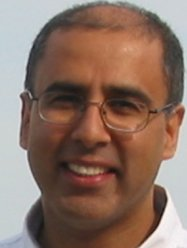
\includegraphics[width=3.5cm]{introduction/images/drdulay.jpg}};
    \end{tikzpicture}
    \centerline{\textbf{Dr Narankar Dulay}}
\end{center}
The module is taught by \href{http://wp.doc.ic.ac.uk/nd/}{Dr Narankar Dulay}.
\\
\\ \textbf{Theory} For weeks 2 $\to$ 10:
\begin{itemize}
    \item Elixir (learning programming language)
    \item Introduction
    \item Reliable Broadcast
    \item FIFO, casual and total order Broadcast
    \item Consensus
    \item Flip Improbability Result
    \item Temporal Logic of Actions
    \item Modelling Broadcast
    \item Modelling Consensus
\end{itemize}

\section{Course Resources}
The \href{https://www.doc.ic.ac.uk/~nd/dal/}{course website} contains all available slides and notes.

\section{Distributed Systems}
\begin{definitionbox}{Distributed System}
    A set of processes connected by a network, communicating by message passing and with no shared physical clock.
    \begin{itemize}
        \item No total order on events by time (no shared clock)
        \item No shared memory.
        \item Network is logical - processes may be on the same OS process, same VM, same machine different machines communicating over a physical network. 
    \end{itemize}
\end{definitionbox}

Distributed systems must contend with the inherit uncertainty (failure, communication delay and an inconsistent view of the system's state) in communication between potentially physically independent processes (fallible machines, networks and software).

\begin{sidenotebox}{Leisle Lamport}
    A computer scientist and mathematician, credited with creating TLA (used on this course), as well as being the initial developer of latex (used for these notes).
    \begin{quote}
        "
            There has been considerable debate over the years 
            about what constitutes a distributed system. It 
            would appear that the following definition has been 
            adopted at SRC:

            A distributed system is one in which the failure of 
            a computer you didn't even know existed can render 
            your own computer unusable.
        "
    \end{quote}
\end{sidenotebox}

\section{Distributed Algorithms}
\begin{tcbraster}[raster columns=2, raster equal height]
    \begin{definitionbox}{Liveness Properties}
        \textit{Something good happens eventually} (Cannot be violated by finite computation)
    \end{definitionbox}
    \begin{definitionbox}{Safety Properties}
        \textit{Nothing bad happens} (Only violated by finite computations)
    \end{definitionbox}
\end{tcbraster}

As liveness properties depend on computation, they can be constrained by a \textit{fairness property}.
\\ \begin{tabular}{l p{.8\textwidth}}
    \textbf{unconditional fairness} & Every process gets its turn infinitely often. \\
    \textbf{strong fairness} & Every process gets its turn infinitely often if it is enabled infinitely often. \\
    \textbf{weak fairness} & Every process gets its turn infinitely often if it is continuously enabled from a particular point in the execution. \\
\end{tabular}

\subsection{Key Aspects}
\begin{enumerate}
    \item {\textbf{The problem}
        Specified in terms of the \textit{safety} and \textit{liveness} properties of the algorithm.
    }
    \item {\textbf{Assumptions made}
        \\ \begin{tabular}{l l}
            Bounds on process delays & (timing assumption) \\
            Types of process failures tolerated & (failure assumption) \\
            Use of reliable message passing & (communication assumption) \\
        \end{tabular}
    }
    \item {\textbf{The algorithm}
        Expresses the solution to \textit{the problem}, given \textit{the assumptions}.
        \begin{itemize}
            \item Must prove the algorithm is correct (satisfies all \textit{safety} and \textit{liveness} properties)
            \item Time and space complexity of the algorithm
        \end{itemize}
    }
\end{enumerate}

\begin{examplebox}{Mutual Exclusion Properties}
    What are the safety, liveness and fairness properties required for mutual exclusion of processes over some critical section?
    \tcblower
    \begin{center}
        \begin{tabular}{l p{.5\textwidth} l}
            \textbf{Safety} & At most one process accesses the critical section. & $(s \| t) \land (s \neq t) \Rightarrow \neg (cs(s) \land cs(t))$ \\
            \textbf{Liveness} & Every request for the critical section is eventually granted. & $req(s) \Rightarrow (\exists t : s \preccurlyeq t \land cs(t))$ \\
            \textbf{Fairness} & Requests are granted in the order. & $\begin{matrix*}[l]
                req\_start(s) \land req\_start(t) \land (s \to t) \\
                \Rightarrow (next\_cs(s) \to next\_cs(t)) \\
            \end{matrix*}$ \\
        \end{tabular}
    \end{center}
    Note that $\preccurlyeq$ is the \textit{happens-before} relation.
\end{examplebox}

\begin{definitionbox}{Concensus}
    \[\text{Processes Propose Values} \to \text{Processes decide on value} \to \text{Agreement Reached}\]
    \begin{center}
        \begin{tabular}{l p{.7\textwidth}}
            \textbf{Agreement Property} & Two correct processes cannot decide on different values. \\
            \textbf{Validity Property} & If all processes propose the same value, then the decided value is the proposed value. \\
            \textbf{Termination Property} & System reaches agreement in finite time. \\
        \end{tabular}
    \end{center}
    Consensus is impossible to solve for a fully asynchronous system, some timing assumptions are required.
\end{definitionbox}

It is difficult to prove the correctness of even simple distributed systems formally. By specifying an abstract model of an algorithm automatic model checkers can be used to verify properties.

\subsection{Timing Assumptions}
\begin{definitionbox}{Asynchronous Systems}
    A system where process execution steps and inter-process communication take arbitrary time.
    \begin{itemize}
        \item No assumptions that processes have physical clocks.
        \item Sometimes useful to use \textit{logical clocks} (used to capture a consistent ordering of events on a virtual timespan)
    \end{itemize}
\end{definitionbox}

\begin{definitionbox}{Synchronous Systems}
    A system containing assumptions on the upper bound timings for executing steps in a process.
    \begin{itemize}
        \item This means there are upper bounds for steps such as receiving messages, sending messages, arithmetic, etc.
        \item Easier to reason about.
        \item Implementation must ensure bounds are always met, this can potentially require very high bounds (so guarantee holds) which reduce performance. \textit{Eventually synchronous models} were created to overcome this.
    \end{itemize}
\end{definitionbox}

\begin{definitionbox}{Eventually Synchronous Systems}
    Mostly synchronous systems. Do not have to \textit{always} meet bounds, and can have periods of asynchronicity.
\end{definitionbox}

\subsection{Failure Classes}
\begin{definitionbox}{Process Failure}
    A process internally fails and behaves incorrectly. Process sends messages it should not, or does not send messages it should.
    \begin{itemize}
        \item Can be caused by a software bug, termination of process by user or OS, OS failure, hardware failure, cyber attack by adversary.
        \item The process may be slowed down to the point it cannot send messages it needs to (or meet some timing assumption)
    \end{itemize}
    \begin{center}
        \begin{tabular}{l l}
            \textbf{Fail-Stop} & Failure can be reliably detected by other processes. \\
            \textbf{Fail-Silent} & Not Fail-Stop. \\
            \textbf{Fail-Noisy} & Failure can be detected, but takes time. \\
            \textbf{Fail-Recovery} & Failing process can recover from failure. \\
        \end{tabular}
    \end{center}
    A process that is not faulty is a \textbf{Correct Process}. 
\end{definitionbox}


\begin{tcbraster}[raster columns=2, raster equal height]
    \begin{definitionbox}{Link Failure}
        A link allowing for processes to communicate is disconnected and remains disconnected.
        \\
        \\ A network connecting machines hosting processes may become partitioned due to a \textit{link failure}
    \end{definitionbox}
    \begin{definitionbox}{Byzantine Failure}
        Also called \textbf{Fail-Arbitrary}, a process exhibits some arbitrary behaviour (can be malicious).
    \end{definitionbox}
\end{tcbraster}
\begin{definitionbox}{Omission Failure}
    \begin{center}
        \begin{tabular}{l l}
            \textbf{Send Omission} & Fails to send all messages required by the algorithm. \\
            \textbf{Receive Omission} & Fails to properly receive all messages required. \\
        \end{tabular}
    \end{center}
\end{definitionbox}

\subsection{Communication Assumptions}
\subsubsection{Asynchronous Message Passing}
Processes continue after sending messages, they do not wait for a message to be delivered. It is possible to build a synchronous message passing abstraction from asynchronous message passing.

\subsubsection{Reliable Message Communication}
Messages are assumed to be conveyed using a reliable medium.
\begin{itemize}
    \item All sent messages are delivered.
    \item No duplicate messages are created.
    \item All delivered messages were sent.
\end{itemize}
\noindent
Network failure is still a concern (breaks assumption), so TCP is used for messages, and more reliable message passing abstractions built on top.
\\
\\ Message delays are bounded, as a timeout is used.

\subsection{Complexity}
Complexity can be characterised using:
\begin{itemize}
    \item Number of messages exchanged.
    \item Size of messages exchanged.
    \item Time taken from the perspective of an external observer, or some clock on a synchronous system.
    \item Memory, CPU time or energy used by processes.
\end{itemize}
